\section{The search through Maching Learning}
\subsection{Model selection}
In this analysis I have chosen to compare 4 different \ac{ML}-models, \ac{FFNN}, \ac{PNN},
\ac{LWTA} and XGBoost. The first three methods are all types of \ac{NN}. I have deliberately 
chosen to focus on \ac{NN} given that there is far more freedom in the design of the architecture
of a \ac{NN}, than compared to a XGboost. Additionally, this was motivated by the selfish reason
being that I found the networks more interesting to study and dissect. Therefor, most of the 
analysis, comparison and discussion is focused on the networks, while XGBoost is included 
as a loose benchmark. 
\\
\subsection{Creating custom layers}
The field of \ac{ML} is one of the most dynamic and fastest growing fields of research
today. This means, that regardless of the brave attempt made by voluntary contributors and
the people at Google \footnote{The developers of TensorFlow}, there will always be 
new and exciting \ac{ML} tools, not yet implemented in their library. This was also 
the case in this thesis. Specifically, in the case of non-dense layers I was forced
to dive into the world of \ac{ML} development and create my own implementation. 
\subsubsection*{Max-out}
TensorFlow have already implemented a very similar layer called MaxPooling1D. This does 
exactly what max-out does, but with minor differences. Additionally, to wanting to avoid 
these differences, I wanted the freedom to experiment with the implementation of the 
layer. The implementation of both max-out and channel-out was done by creating a custom 
activation function which is called inside a dense-layer. In the case of max-out, it is 
inside the activation function that the down scaling of nodes happens. 
\\
In the code listing, \ref{lst:max_out} I have included the code implementation of the
activation function used to create the max-out layer. The listing shows how the function
takes the input from the previous layer, defines the new shape of what will become the 
output, groups the nodes in the size defined by number of units, then return an output 
which includes only the largest activated node from each unit. By using this function 
in a dense-layer, said layer will act as a max-out layer. 
\lstset{style=Python}
\begin{lstlisting}[caption={Python implementation for the custom activation function used to define the max-out layer.},captionpos=b, label={lst:max_out}]
def call(self, inputs: tf.Tensor) -> tf.Tensor:
    # Passing input through weight kernel and adding bias terms
    inputs = gen_math_ops.MatMul(a=inputs, b=self.kernel)
    inputs = nn_ops.bias_add(inputs, self.bias)

    num_inputs = inputs.shape[0]
    if num_inputs is None:
        num_inputs = -1
    num_competitors = self.units // self.num_groups
    new_shape = [num_inputs, self.num_groups, num_competitors]

    # Reshaping outputs such that they are grouped correctly
    inputs = tf.reshape(inputs, new_shape)
    # Finding maximum activation in each group
    outputs = tf.math.reduce_max(inputs, axis=-1,keepdims=True)

    counter = tf.where(tf.equal(inputs, outputs), outputs, 0.)
    # Reshaping outputs to original input shape
    self.counter = tf.reshape(counter, [num_inputs, self.units])

    return tf.reshape(outputs,[num_inputs, self.num_groups])   
\end{lstlisting}
\subsubsection*{Channel-out}
For the activation function defined to create the channel-out layer, I again grouped
the nodes similarly as I did for max-out. Instead of returning the largest value from each 
unit, I used TensorFlow's function, $tf.greater\_equal$ to create a tensor with booleans. The 
booleans are chosen by comparing each unit to the largest value in that unit. By multiplying 
this tensor to the original input, I am left with the desired result of a tensor containing 
the largest activated nodes along with the rest whom are now set to zero. 
\lstset{style=Python}
\begin{lstlisting}[caption={Python implementation for the custom activation function used to define the channel-out layer.},captionpos=b, label={lst:channel_out}]
def channel_out(inputs, num_units = 200, axis=None, training=None):
    # Calculate the new shape of the layer after max_out.
    shape = inputs.get_shape().as_list()
    if shape[0] is None:
        shape[0] = -1
    if axis is None:  # Assume that channel is the last dimension
        axis = -1
    num_channels = shape[axis]
    
    if num_channels % num_units:
        raise ValueError('Number of features is not a multiple of num_units')
    shape[axis] = num_units
    shape += [num_channels // num_units]
    grouped = tf.reshape(inputs, shape)
    # Calculate the largest value in each unit and discard 
    top_vals = tf.reduce_max(grouped, -1, keepdims=True)
    isMax = tf.reshape(tf.greater_equal(grouped, top_vals), [shape[0], num_channels])
    output = tf.multiply(tf.cast(isMax,tf.float32), inputs)
    return output  
\end{lstlisting}
\subsection{Model Architecture}
When choosing network architecture, there are several ways to go about it. One way is to apply a grid search.
A grid search is simply defining a grid of parameters to test, then running through all combinations and 
choosing the highest performer. With a sufficient amount of tests, a grid search should converge towards 
an optimal architecture. Grid search is very common and there exists a large range of very complex varieties \cite{GS}.
For my analysis I choose not to perform a grid search, for several reasons. The first being interpretability.
Understanding a \ac{NN} is already hard, allowing for complex and unique architectures would only add another layer
of mysticism. The second is the size of the data set. The larger the data set, the larger the amount of data 
would be needed to adequately perform tests for each combination of parameters. Not only is this time-consuming,
but trying to mediate this issue could lead to poor performance. The third and most important reason is that 
I wanted to experiment with the architectures. By manually tuning the parameters, I was able to achieve a far 
better understanding of the final architecture. 

\begin{figure}
    \centering
    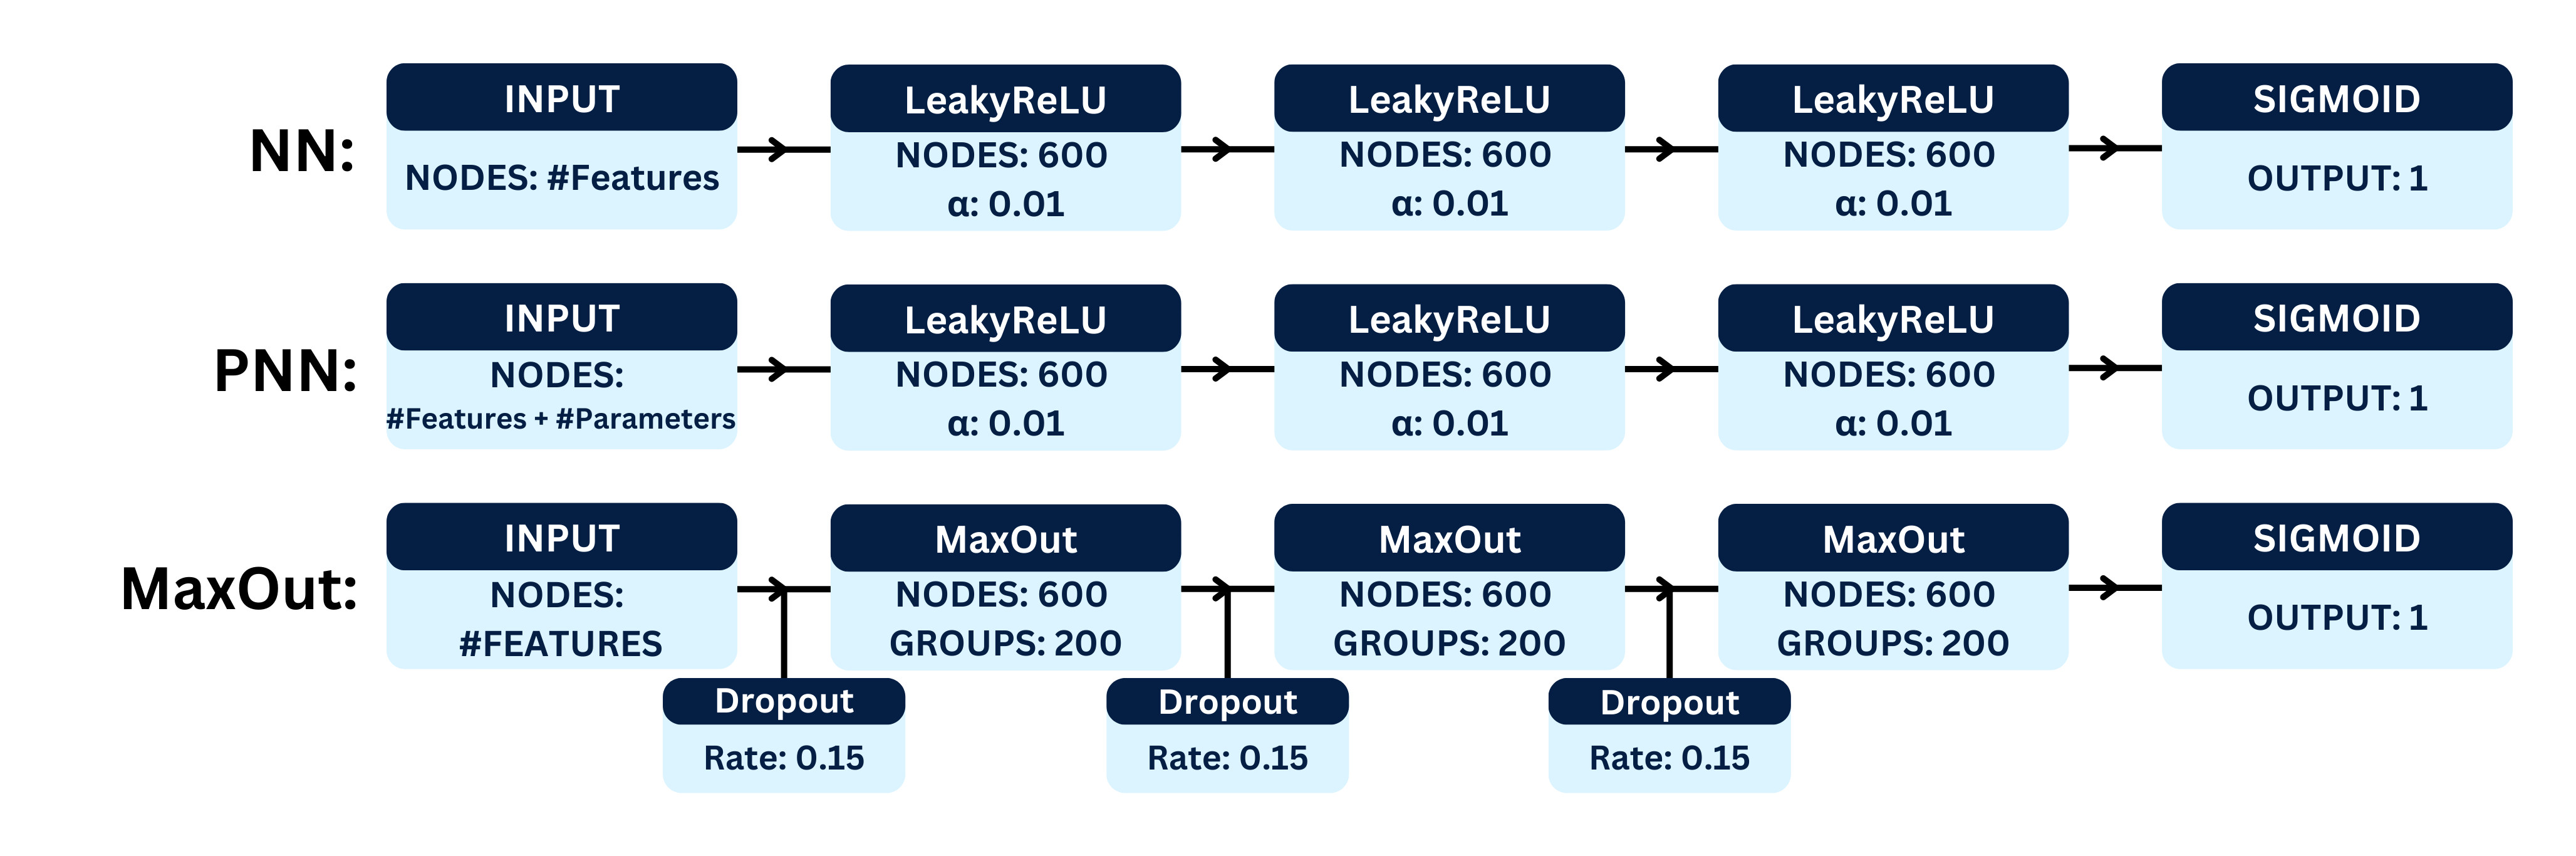
\includegraphics[width=1\textwidth]{Figures/Illustrations/architecture.png}
    \caption{A visual summary of the workflow and framework use for the 
    computational analysis. }
    \label{fig:arch}
\end{figure}
